%\chapter{orbits}\label{sec:orbits}
\section{Orbit of the LMC}\label{sec:orbits}

\subsection{ICs}

The initial conditions are found integrating the galaxies backwards
in time from their present day observed positions and velocity \citep{K13},
 the values are resumed in table \ref{tab:LMCrv}.

\begin{table}[H]
\begin{center}
\begin{tabular}{c c c}
\hline
\hline
x(kpc) & y(kpc) & z(kpc) \\
& & & \\
\hline
 vx($km s^{-1}$) & vy($km s^{-1}$) & vz($km s^{-1}$) \\
\hline
-57 \pm 13 & -226 \pm 15 & 221 \pm 19
\end{tabular}
\end{center}
\caption{\label{tab:LMCrv}}
\end{table}

Fig. shows the orbits of all the models.

\subsection{Resolution tests}

In order to compute the orbit, the center of mass of the galaxies
have to be computed at each time step. The center of mass is usually
computed using the minimum of the potential, in this case the minimum
of the potential is that corresponding to the most bound particle.
Fig \ref{fig:res} shows both computations.

\begin{figure}[H]
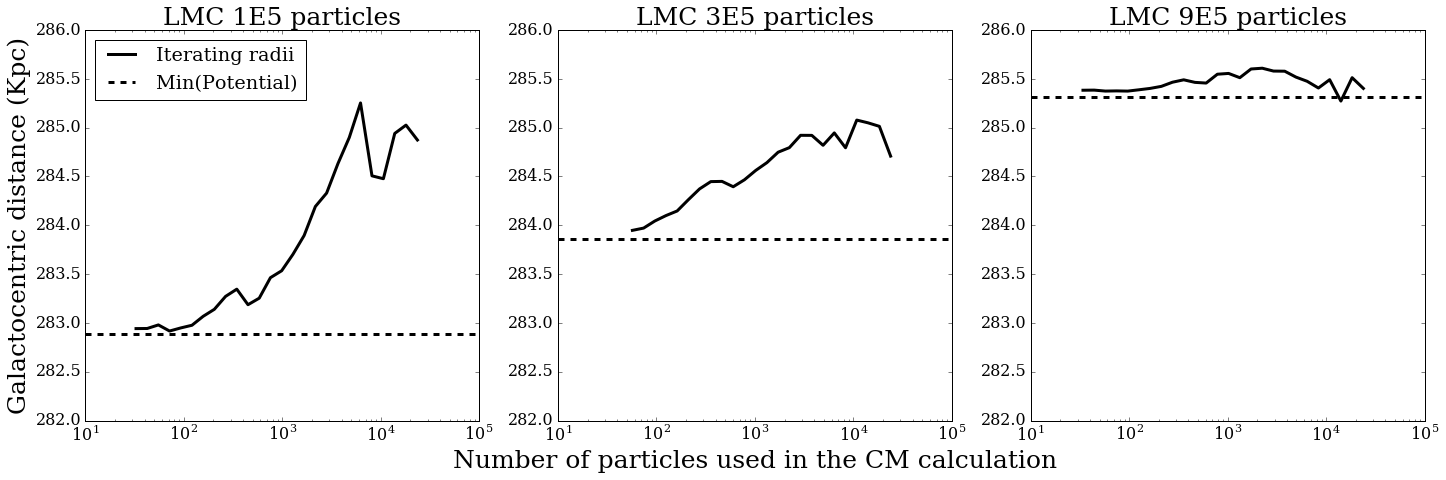
\includegraphics[scale=0.3]{resolution_test.png}
\caption{The code that reproduces this plot is available at:
\href{https://github.com/jngaravitoc/LMC-MW/blob/master/code/CMResolution-test.ipynb}{Github}\label{fig:res}}
\end{figure}


